\documentclass[]{elsarticle} %review=doublespace preprint=single 5p=2 column
%%% Begin My package additions %%%%%%%%%%%%%%%%%%%
\usepackage[hyphens]{url}



\usepackage{lineno} % add
\providecommand{\tightlist}{%
  \setlength{\itemsep}{0pt}\setlength{\parskip}{0pt}}

\biboptions{sort&compress} % For natbib
\usepackage{graphicx}
\usepackage{booktabs} % book-quality tables
%%%%%%%%%%%%%%%% end my additions to header

\usepackage[T1]{fontenc}
\usepackage{lmodern}
\usepackage{amssymb,amsmath}
\usepackage{ifxetex,ifluatex}
\usepackage{fixltx2e} % provides \textsubscript
% use upquote if available, for straight quotes in verbatim environments
\IfFileExists{upquote.sty}{\usepackage{upquote}}{}
\ifnum 0\ifxetex 1\fi\ifluatex 1\fi=0 % if pdftex
  \usepackage[utf8]{inputenc}
\else % if luatex or xelatex
  \usepackage{fontspec}
  \ifxetex
    \usepackage{xltxtra,xunicode}
  \fi
  \defaultfontfeatures{Mapping=tex-text,Scale=MatchLowercase}
  \newcommand{\euro}{€}
\fi
% use microtype if available
\IfFileExists{microtype.sty}{\usepackage{microtype}}{}
\bibliographystyle{elsarticle-harv}
\usepackage{longtable}
\ifxetex
  \usepackage[setpagesize=false, % page size defined by xetex
              unicode=false, % unicode breaks when used with xetex
              xetex]{hyperref}
\else
  \usepackage[unicode=true]{hyperref}
\fi
\hypersetup{breaklinks=true,
            bookmarks=true,
            pdfauthor={},
            pdftitle={Codebook: Unveiling the ecosystem of science},
            colorlinks=false,
            urlcolor=blue,
            linkcolor=magenta,
            pdfborder={0 0 0}}
\urlstyle{same}  % don't use monospace font for urls

\setcounter{secnumdepth}{0}
% Pandoc toggle for numbering sections (defaults to be off)
\setcounter{secnumdepth}{0}
% Pandoc header



\begin{document}
\begin{frontmatter}

  \title{Codebook: Unveiling the ecosystem of science}
    \author[a]{Nicolas Robinson-Garcia\corref{c1}}
   \ead{N.Robinson@tudelft.nl} 
   \cortext[c1]{Corresponding author}
    \author[b]{Rodrigo Costas}
  
  
    \author[b]{Thed N. van Leeuwen}
  
  
    \author[a]{Tina Nane}
  
  
      \address[a]{Applied Mathematics (DIAM), TU Delft, Delft, Netherlands}
    \address[b]{CWTS, Leiden University, Leiden, Netherlands}
  
  \begin{abstract}
  There is increasing evidence on the misuse and abuse of quantitative
  indicators in the current scientific reward system. Alternatively, more
  qualitative approaches, use of case studies or the design of indicators
  more sensitive to societal and scientific needs have been suggested. In
  this article we analyze the bases of such criticisms and motivations for
  changing the reward system by focusing on the assessment of individuals.
  We explore alternative models proposed or in use and identify common
  characteristics. Based on this we propose a valuation model by which we
  can systematically organize and prioritize performative aspects of
  scientists and consider other factors which may affect or might relevant
  for research policy. We finally test our model in a series of case
  studies based on six academic units.
  \end{abstract}
  
 \end{frontmatter}

Here I describe the selection of case studies and the data retrieval
process and description of sources. The purpose of this is to show that
1) there are indeed a variety of different profiles, 2) these profiles
co-exist and complement each other, 3) the diversity and typologies of
profiles is field dependent, 4) personal features are key to understand
this diversity. Here we emphasize two specific personal features: age
and gender. Some of the research questions that could be answered
descriptively are the following:

\begin{enumerate}
\def\labelenumi{\arabic{enumi}.}
\tightlist
\item
  \emph{Is there team science?}
\end{enumerate}

\begin{enumerate}
\def\labelenumi{\roman{enumi}.}
\tightlist
\item
  \emph{Are these teams stable over time?} Some data that could be
  retrieved from WoS
\end{enumerate}

\begin{verbatim}
-   Cluster_id
-   All classic bibliometric indicators
-   Number of collaborators from same institution
-   Number of external collaborators
-   Number of collaborators from same institution by publication
-   Number of external collaborators by publication
\end{verbatim}

\begin{enumerate}
\def\labelenumi{\roman{enumi}.}
\setcounter{enumi}{1}
\tightlist
\item
  \emph{Is there activity visible through co-authorship?} Check groups
  identified with manual checking in the web and maybe interviews
\end{enumerate}

\begin{enumerate}
\def\labelenumi{\arabic{enumi}.}
\setcounter{enumi}{1}
\tightlist
\item
  \emph{Do research teams operate in a coordinated way?} Here it would
  be interesting to understand dependence relationship. Nederhof \& van
  Raan (1993) refer to the star effects as what happens when a PI
  retires and the research group disappears. Here we should go beyond
  bibliometrics and see if there is someone in charge of the funding,
  someone of hiring and finding opportunities, someone who is more of a
  public face, etc. Also it would be interesting to use network analysis
  to determine authorities, hubs, etc. and contrast with their judgment.
  Some variables from WoS and interivews plus manually cheking:
  authorship position (WoS); acknowledgments data (WoS); clusters from
  Ludo's subject classification to identify areas of specialization per
  subject (WoS); social media activity; Google Scholar data.
\end{enumerate}

\begin{enumerate}
\def\labelenumi{\roman{enumi}.}
\tightlist
\item
  \emph{Do they have a common research agenda?}
\item
  \emph{How is this agenda established?}
\end{enumerate}

\begin{enumerate}
\def\labelenumi{\arabic{enumi}.}
\setcounter{enumi}{2}
\tightlist
\item
  \emph{How does team science affect individual trajectories?}
\end{enumerate}

\begin{enumerate}
\def\labelenumi{\roman{enumi}.}
\tightlist
\item
  \emph{How is credit shared?}
\item
  \emph{What is the relation between the role exerted and academic
  status?} A cohort analysis?
\item
  \emph{How is continuity of supporting scientists ensured?} Probably
  also from interviews. How do scholars change from institution or are
  maintained if they are not able to `make the next step'.
\end{enumerate}

\hypertarget{selection-of-case-studies}{%
\subsection{Selection of case studies}\label{selection-of-case-studies}}

The identification of research groups is done bibliometrically and based
on Web of Science publications. For this I have selected all
publications between 2008 and 2017 by LUMC, Leiden University or TU
Delft. The following table includes some descriptives. Here I must note
that researchers belonging to institutions are not based on the specific
affiliation linkage of docs (which uses the Leiden Ranking affiliation
already cleaned up), but based on \texttt{cluster\_id} with either of
the three institutions as their main or alternative address. This should
be checked to see if there is a way to link to the \texttt{cluster\_id}
organizations to the cleaned affiliations from Leiden Ranking. I had to
clean up this data myself. In any case this should not be a concern for
the selection of case studies.

\begin{longtable}[]{@{}lccc@{}}
\toprule
& TU Delft & Leiden Univ & LUMC\tabularnewline
\midrule
\endhead
Publications & 24,233 & 49,149 & 3,188\tabularnewline
Researchers & 9,975 & 14,116 & 279\tabularnewline
Collaborators & 34,409 & 117,307 & 14,153\tabularnewline
Mean au/p & 4.7 & 9.6 & 10.1\tabularnewline
Median au/p & 4 & 6 & 8\tabularnewline
Sd au/p & 5.4 & 31.5 & 18.7\tabularnewline
\bottomrule
\end{longtable}

The next figure shows the distribution of papers based on the number of
authors by paper (A) and the thematic profile of each of the three
institutions. Leiden University is the largest of the three institutions
with a more comprehensive portfolio, although mostly focues on
Biomedical Sciences and Social Sciences. This focus on biomedical
sciences is obviously more noticeable in the case of LUMC, although it
still has some pubications in fields of the social sciences, mostly
related with Public Health. Finally, TU Delft shows a profile focused on
Phisics, Engineering and Mathematics. While there might be an overlap
between LUMC and Leiden University, the high preponderance of biomedical
literature might also be due to a close relation between these
universities.

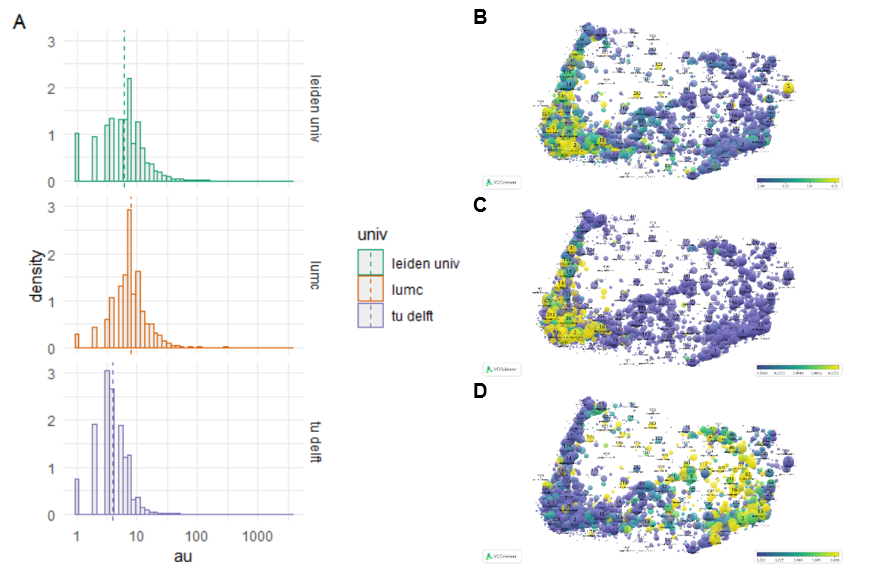
\includegraphics[width=2.97in]{figs/histogram-profiles}

Six case studies will be selected. Three for each university and two by
field. The purpose of this is not only to identify differences by
discipline but also by institutional type. The fields are:

\begin{enumerate}
\def\labelenumi{\arabic{enumi}.}
\tightlist
\item
  Physics and Engineering
\item
  Social Sciences and Humanities
\item
  Biomedical Sciences
\end{enumerate}

Following I include the collaboration networks for each university and
field. I have included a threshold of at least 10 publications by
\texttt{cluster\_id}, filtered by the giant component and calculated the
betweenness centrality of each node. I have selected as seed researcher
the one with the highest centrality.

\hypertarget{physics-engineering}{%
\subsubsection{Physics \& Engineering}\label{physics-engineering}}

\hypertarget{tu-delft}{%
\paragraph{1. TU Delft}\label{tu-delft}}

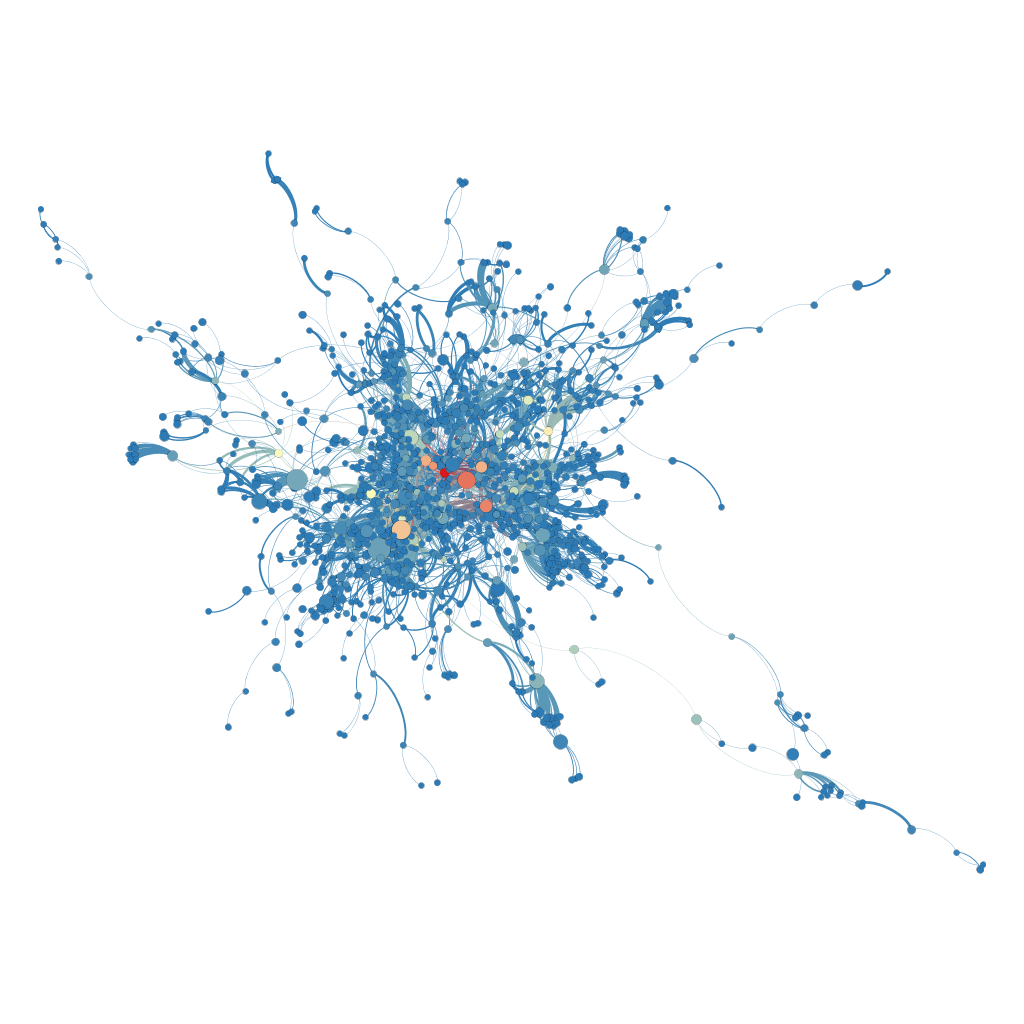
\includegraphics[width=3.41in]{figs/tu_phys_betweenness}

\emph{Notes:}

\begin{itemize}
\tightlist
\item
  1260 nodes (21.9\% visible); 4702 edges (27.1\% visible).
\item
  \texttt{cluster\_id} with highest betweenness = 33800547; Betweenness
  centrality: 0.11; Total publications = 159; Age = 32
\item
  Name: Frans D. Tichelaar; First year: 1986; Last year: 2018
\item
  PURE:
  https://pure.tudelft.nl/portal/en/persons/fd-tichelaar(56299c58-b6ec-478b-b188-b8744b69d954).html
\item
  Institution: http://nchrem.nl/people/dr-ir-f-d-tichelaar-frans/
\end{itemize}

\hypertarget{leiden-univ}{%
\paragraph{2. Leiden Univ}\label{leiden-univ}}

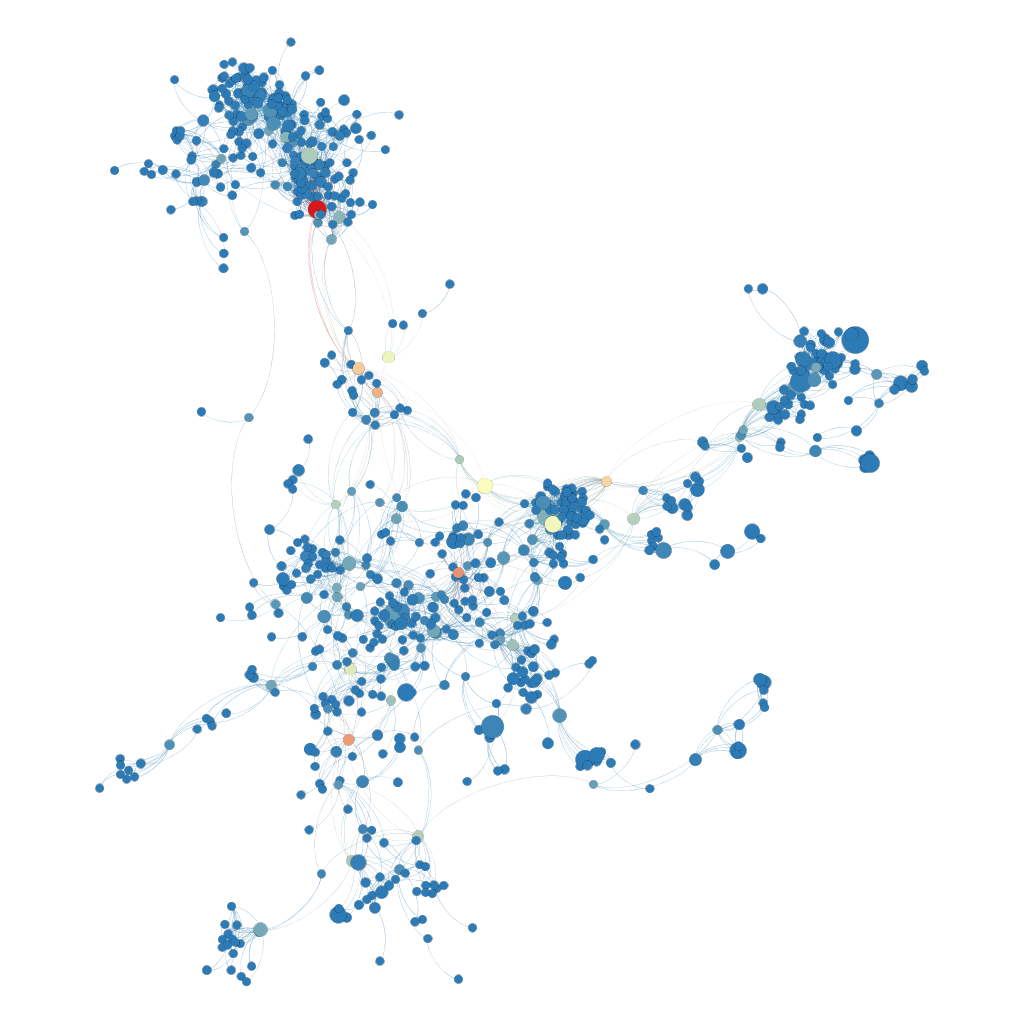
\includegraphics[width=3.41in]{figs/lu_phys_betweenness}

\emph{Notes:}

\begin{itemize}
\tightlist
\item
  765 nodes (35.1\% visible); 3409 edges (40.6\% visible).
\item
  \texttt{cluster\_id} with highest betweenness = 25501410; Betweenness
  centrality: 0.23; Total publications = 590; Age = 38
\item
  Name: Ewine F. van Dishoeck; First year: 1980; Last year: 2018
\item
  Institution:
  https://local.strw.leidenuniv.nl/people/touchscreen2/persinline.php?id=16
\item
  Personal website:
  https://home.strw.leidenuniv.nl/\textasciitilde{}ewine/
\end{itemize}

\hypertarget{biomedical-and-health-sciences}{%
\subsubsection{Biomedical and Health
Sciences}\label{biomedical-and-health-sciences}}

\hypertarget{tu-delft-1}{%
\paragraph{1. TU Delft}\label{tu-delft-1}}

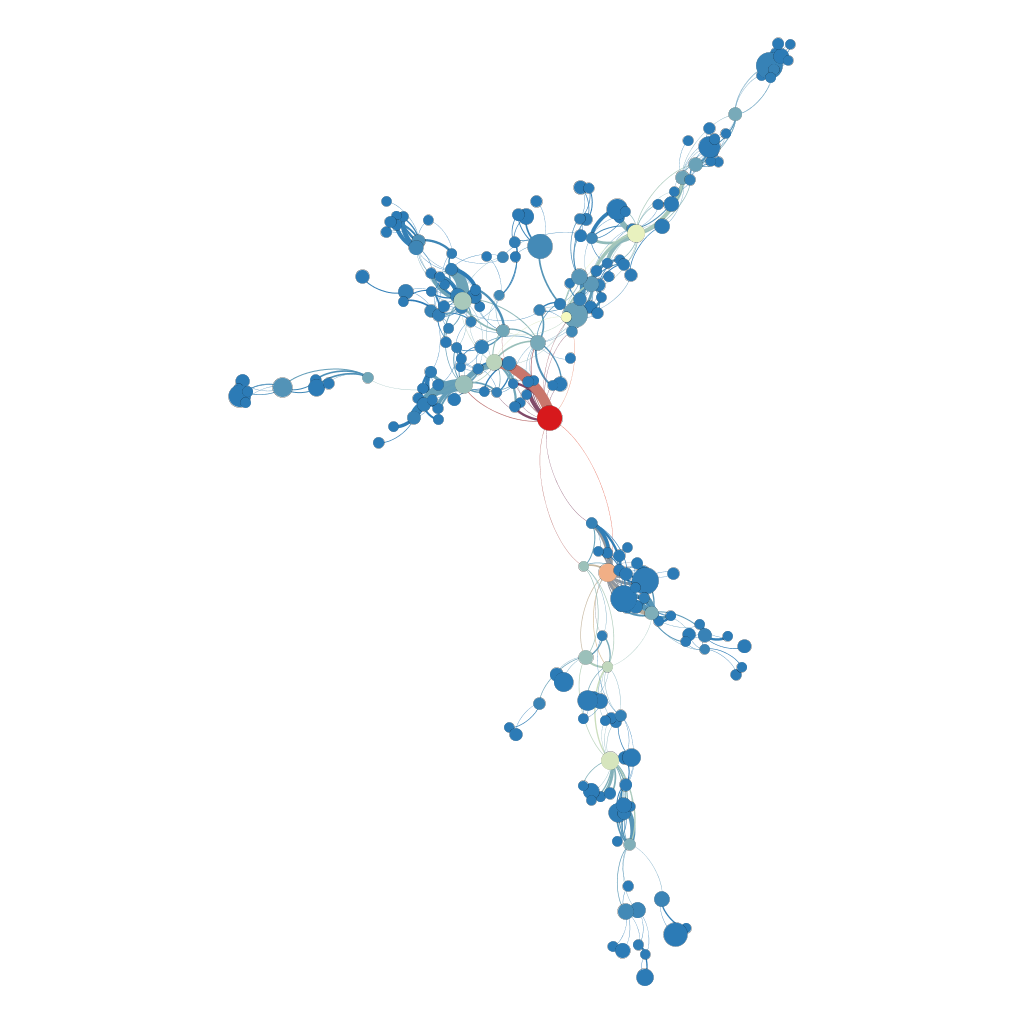
\includegraphics[width=3.41in]{figs/tu_bio_betweenness}

\emph{Notes:}

\begin{itemize}
\tightlist
\item
  214 nodes (18.9\% visible); 615 edges (25.49\% visible).
\item
  \texttt{cluster\_id} with highest betweenness = 43204348; Betweenness
  centrality: 0.50; Total publications = 341; Age = 31
\item
  Name: Harrie H. Weinans; First year: 1987; Last year: 2018
\item
  Google Profile:
  https://scholar.google.com/citations?user=di4NUp8AAAAJ\&hl=en
\item
  PURE:
  https://pure.tudelft.nl/portal/en/persons/hh-weinans(f31bd75b-1863-4202-b64b-7356538284a7)/publications.html
\item
  Co-affiliated to UMC Utrecht and TU Delft.
\end{itemize}

\hypertarget{leiden-univ-1}{%
\paragraph{2. Leiden Univ}\label{leiden-univ-1}}

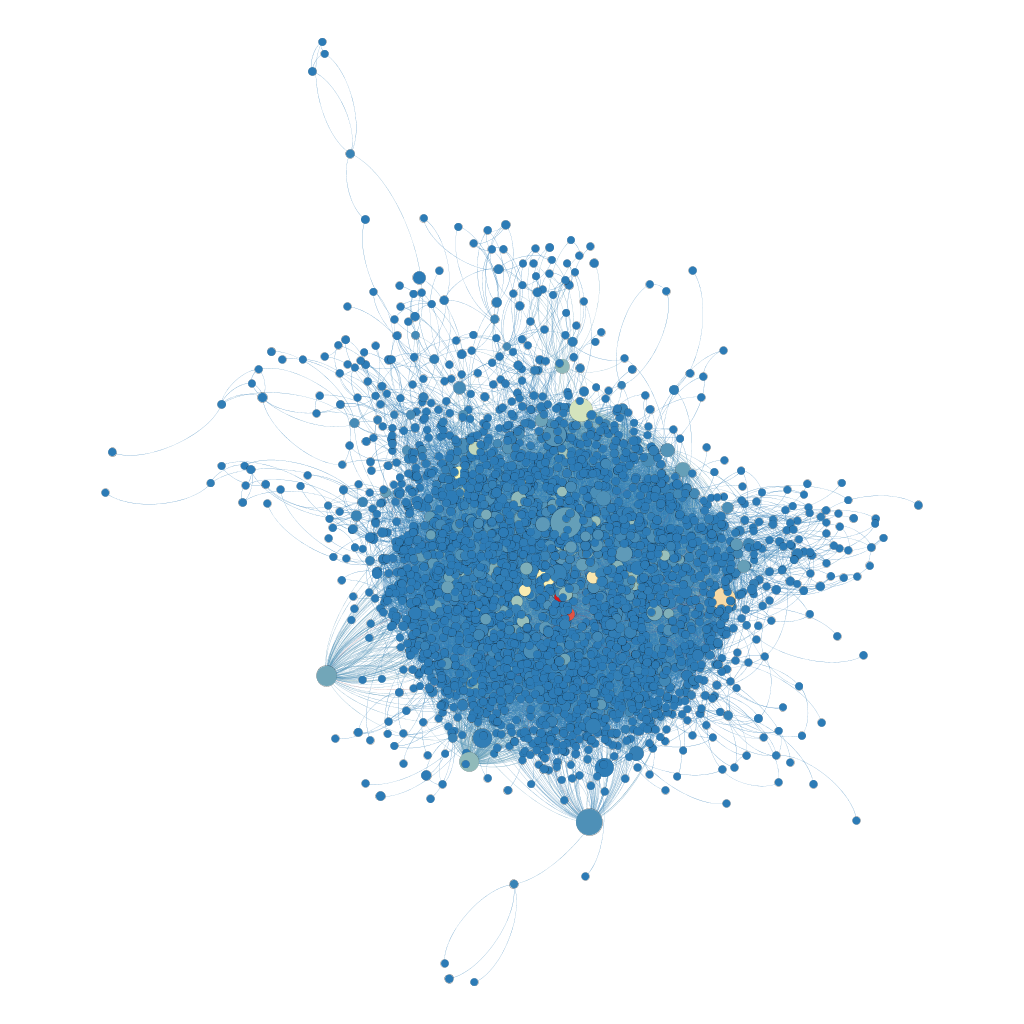
\includegraphics[width=3.41in]{figs/lu_bio_betweenness}

\emph{Notes:}

\begin{itemize}
\tightlist
\item
  Due to the density of the network the selected node can scarcely be
  seen.
\item
  3304 nodes (38.8\% visible); 43647 edges (59.6\% visible).
\item
  \texttt{cluster\_id} with highest betweenness = 19936939; Betweenness
  centrality: 0.47; Total publications = 185; Age = 27
\item
  Name: Ron Wolterbeek; First year: 1991; Last year: 2018
\item
  Institution: https://www.lumc.nl/org/bds/medewerkers/rwolterbeek
\item
  Affiliated to LUMC.
\end{itemize}

\hypertarget{social-sciences-and-humanities}{%
\subsubsection{Social Sciences and
Humanities}\label{social-sciences-and-humanities}}

\hypertarget{tu-delft-2}{%
\paragraph{1. TU Delft}\label{tu-delft-2}}

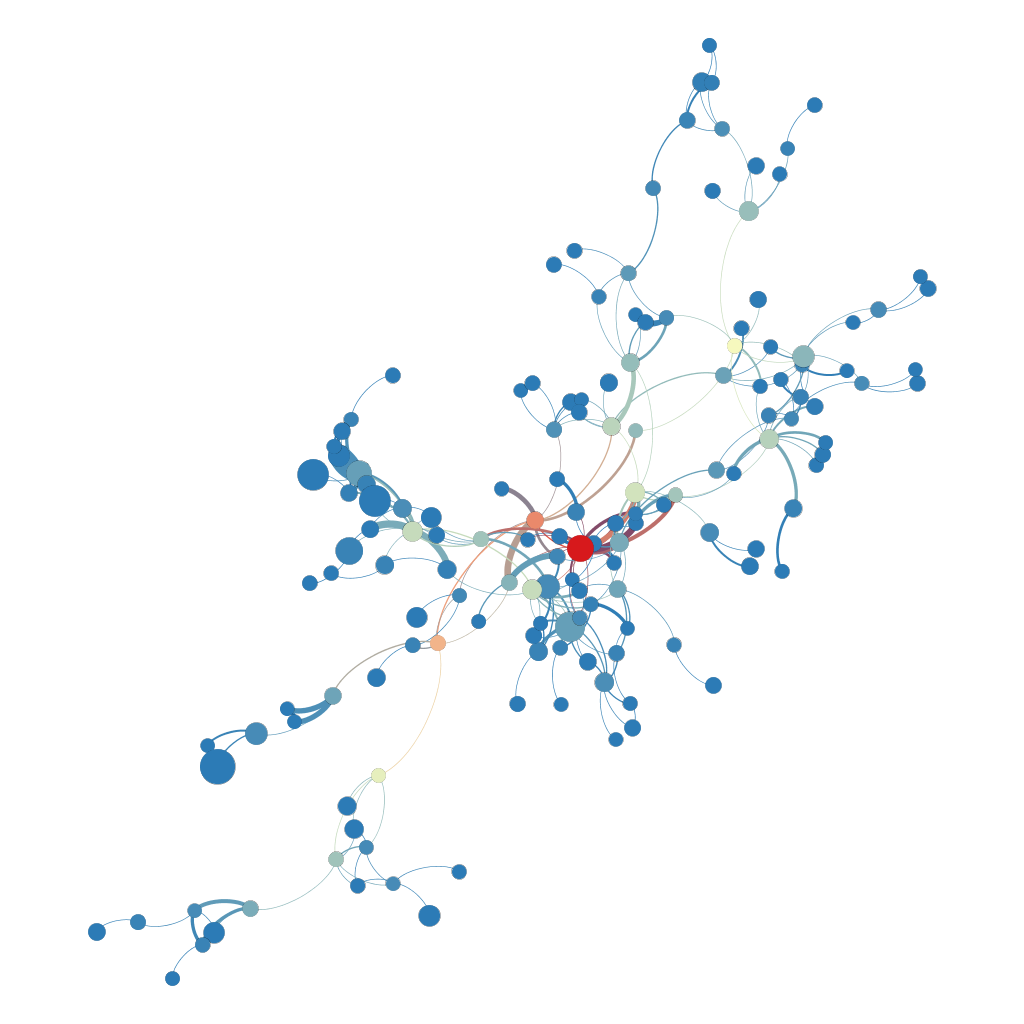
\includegraphics[width=3.41in]{figs/tu_soc_betweenness}

\emph{Notes:}

\begin{itemize}
\tightlist
\item
  151 nodes (12.6\% visible); 281 edges (15.8\% visible).
\item
  \texttt{cluster\_id} with highest betweenness = 12392841; Betweenness
  centrality: 0.41; Total publications = 134; Age = 18
\item
  Name: Bert van Wee; First year: 1999; Last year: 2018
\item
  Google Profile:
  https://scholar.google.es/citations?user=dYUiqMYAAAAJ\&hl=en
\item
  Institution:
  https://www.tudelft.nl/en/tpm/about-the-faculty/departments/engineering-systems-and-services/people/full-professors/profdr-gp-bert-van-wee/
\end{itemize}

\hypertarget{leiden-univ-2}{%
\paragraph{2. Leiden Univ}\label{leiden-univ-2}}

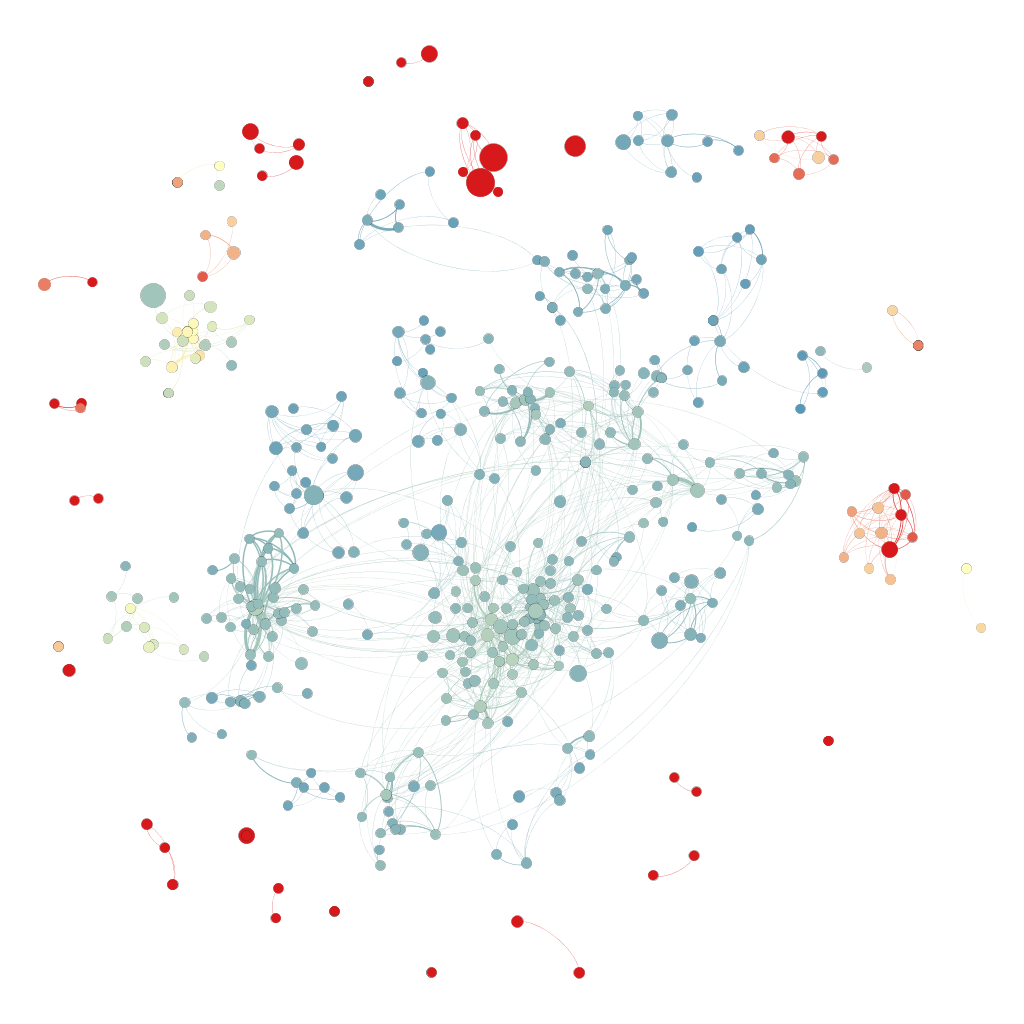
\includegraphics[width=3.41in]{figs/lu_soc_betweenness}

\emph{Notes:}

In this case, the selection of the seed researcher was not based on
network indicator. The network above has the OpenOrd layout (instead of
Yi ) and K-Core=1 group. The main issue here is that this field is
largely populated by biomedical scientists and psychologists and
psychiatrists, fields which are not good representations of Social
Sciences and Humanities. What I have done is looked at those pairs of
scholars with the highest shares of co-authored papers and go down the
list until I found someone who was not from these fields nor from CWTS
(Ludo and Nees are the third pair with more co-authored papers)

\begin{itemize}
\tightlist
\item
  478 nodes (26.5\% visible); 1294 edges (43.1\% visible).
\item
  \texttt{cluster\_id} selected = 36871407; Betweenness centrality:
  0.00; Total publications = 78; Age = 18
\item
  Name: Judi Mesman; First year: 2000; Last year: 2018
\item
  Institution:
  https://www.universiteitleiden.nl/en/staffmembers/judi-mesman/publications\#tab-1
\item
  Lab1: http://www.diversityinparenting.nl/
\item
  Lab2: https://www.societalchallengeslab.com/
\end{itemize}

\hypertarget{expansion-from-seed-to-complete-team}{%
\subsection{Expansion from seed to complete
team}\label{expansion-from-seed-to-complete-team}}

Based on the six individuals selected in the first phase. I know search
for their complete research team. The data retrieval process started on
March, 2019. Here I include for each case how I have proceeded.

\hypertarget{physics-engineering---tu-delft}{%
\subsubsection{Physics \& Engineering - TU
Delft}\label{physics-engineering---tu-delft}}

Dr.~Ir. F.D. Tichelaar belongs to the National Centre for High
Resolution Electron Microscopy. According to its website, he is not the
head of the institute which is formed by 9 researchers (5 staff and 4
researchers and post docs)

\hypertarget{physics-engineering---leiden-univ}{%
\subsubsection{Physics \& Engineering - Leiden
Univ}\label{physics-engineering---leiden-univ}}

Prof.~Ewine van Dishoeck belongs to the Leiden Observatory. According to
its website, there are 179 workers: 33 are staff members, 50 postdocs,
63 PhD students and 26 supporting staff.

\hypertarget{biomedical-sciences---tu-delft}{%
\subsubsection{Biomedical Sciences - TU
Delft}\label{biomedical-sciences---tu-delft}}

Harrie H. Weinans is associate professor at UMC Utrecht in the
department of Orthopaedics and Professor at TU Delft at the
Biomechanical Engineering department. Here information is gathered from
TU Delft. He is a parttime professor. Here I will not include the whole
department, but only researchers working on the Biomaterials \& Tissue
Biomechanics group. Only supporting staff assigned to this group is
included.

\hypertarget{biomedical-sciences---leiden-university}{%
\subsubsection{Biomedical Sciences - Leiden
University}\label{biomedical-sciences---leiden-university}}

Ron Wolterbeek is first-line consultant in the area of Medical
Statistics at LUMC. I could not find him actually in the staff page, so
decided to look into the staff included there. There is not much about
him in the Internet other than his publications.

\hypertarget{social-sciences-and-humanities---tu-delft}{%
\subsubsection{Social Sciences and Humanities - TU
Delft}\label{social-sciences-and-humanities---tu-delft}}

Bert van Wee is professor in Transport Policy at the department of
Engineering Systems and Services. In this case I do not find anything as
research teams or groups and hence I am including the whole department.

\hypertarget{social-sciences-and-humanities---leiden-univ}{%
\subsubsection{Social Sciences and Humanities - Leiden
Univ}\label{social-sciences-and-humanities---leiden-univ}}

Judi Mesman is dean of Leiden University College The Hague and professor
of the interdisciplinary study of societal challenges. She directs the
Societal Challenges Lab which is part of both the Faculty of Governance
and global Affairs and the Faculty of Social Sciences at Leiden
University. This case study is based on her lab.

\hypertarget{data-sources}{%
\subsection{Data sources}\label{data-sources}}

Data sources are selected based on dimensions from the \emph{valuation
model}. Following I include the main ones selected:

\begin{itemize}
\item
  \textbf{CWTS-Web of Science.} Publication and citation indicators are
  retrieved since 1980 or first publication to 2018 by matching
  individual to \texttt{cluster\_id} following the author name
  disambiguation developed by Caron \& van Eck (2014).
\item
\end{itemize}

\pagebreak

\hypertarget{references}{%
\section{References}\label{references}}


\end{document}


